\documentclass[11pt]{article}

% ---------- Packages (per course conventions) ----------
\usepackage[margin=1in]{geometry}
\usepackage{graphicx}
\usepackage{float}
\usepackage{booktabs}
\usepackage{siunitx}
\usepackage{amsmath}
\usepackage{amssymb}
\usepackage{tikz}
\usetikzlibrary{arrows.meta,patterns,calc,decorations.pathmorphing}
\usepackage{tcolorbox}
\usepackage{enumitem}
\usepackage{xcolor}
\usepackage{hyperref}
\hypersetup{colorlinks=true, linkcolor=black, urlcolor=blue}

\setlength{\parindent}{0pt}
\setlength{\parskip}{5pt}

\newcommand{\assignmentNumber}{4}
\newcommand{\assignedDate}{2 Oct 2026}
\newcommand{\dueDate}{8 Oct 2026 (11:59pm, Moodle)}

% ---------- Boxed-answer helper ----------
\newtcolorbox{finalanswer}{
    colback=white, colframe=black, boxrule=1pt,
    title=Answer, fonttitle=\bfseries, coltitle=black,
    colbacktitle=white
}

\newcommand{\probhead}[2]{%
    \clearpage
    \section*{Problem #1}
    \textbf{Given / Find:} #2
    \par\textbf{Sketch:}\par
}

\begin{document}

% =========================================================
% COVERSHEET
% =========================================================
\begin{titlepage}
    \centering
    \vspace*{2cm}
    {\LARGE \bfseries ENGR 225: Mechanics 1} \\[0.3cm]
    {\Large Homework Coversheet} \\[0.3cm]
    {\large Assoc.\ Prof.\ Clayton Byers} \\[2cm]

    \begin{flushleft}
        \Large
        \textbf{NAME:} \underline{\hspace{0.5cm}Sean Balbale\hspace{4cm}} \\[1cm]
        \textbf{DATE:} \underline{\hspace{0.5cm}10/8/2026\hspace{4cm}} \\[1cm]
        \textbf{ASSIGNMENT:} \underline{\hspace{0.5cm}Homework 4\hspace{3.2cm}} \\[2cm]
    \end{flushleft}

    \large
    \textbf{Level of involvement of AI, LLMs, or related tools in the completion of this assignment:}

    \vspace{1cm}

    \begin{flushleft}
        \Large
        $\square$ \quad None \\[0.7cm]
        $\blacksquare$ \quad Minor \\[0.7cm]
        $\square$ \quad Major \\[0.7cm]
        $\square$ \quad Extensive \\[1.5cm]
    \end{flushleft}

    \normalsize
    \textit{Mark the box that applies (e.g., replace $\square$ with $\blacksquare$, or type an X beside it, before compiling/printing). Your disclosure does not affect your grade -- it keeps you accountable for the work you are doing.}

\end{titlepage}

% =========================================================
% HOMEWORK HEADER
% =========================================================
% \section*{ENGR 225 -- Homework \assignmentNumber}
% \textbf{Assigned:} \assignedDate \hfill \textbf{Due:} \dueDate

% \vspace{0.3cm}
% \textit{Formatting per course guidelines: each problem on its own page, with problem summary, labeled sketch, governing equations, units carried throughout, results to 3 significant figures, and a clearly boxed final answer.}

% =========================================================
% PROBLEM 1
% =========================================================
\probhead{1}{Cantilever beam with a 6 kN load at mid-span and a 4 kN force at $30^\circ$ below horizontal on the end of the inclined segment. Find $A_x$, $A_y$, $M_A$.}

\begin{center}
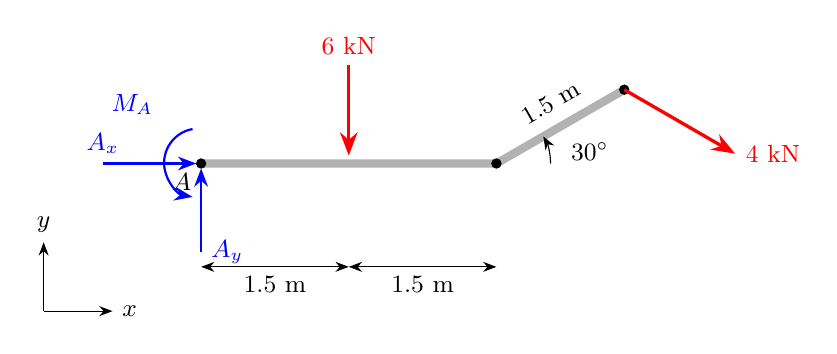
\begin{tikzpicture}[scale=1.25,>=Stealth,font=\small]
  \draw[line width=3pt,gray!60] (0,0)--(3,0)--(4.299,0.75);
  \fill (0,0) circle(1.5pt) node[below left]{$A$};
  \fill (3,0) circle(1.5pt);
  \draw[->,very thick,red] (1.5,1.0)--(1.5,0.08) node[pos=0,above]{$6$ kN};
  \fill (4.299,0.75) circle(1.5pt);
  \draw[->,very thick,red] (4.299,0.75)--++(-30:1.3) node[right]{$4$ kN};
  % reactions (assumed positive directions)
  \draw[->,thick,blue] (-1.0,0)--(-0.05,0) node[pos=0,above]{$A_x$};
  \draw[->,thick,blue] (0,-0.9)--(0,-0.05) node[pos=0,right]{$A_y$};
  \draw[->,thick,blue] (-0.087,0.35) arc (100:260:0.35);
  \node[blue] at (-0.7,0.6) {$M_A$};
  % dimensions
  \draw[<->] (0,-1.05)--(1.5,-1.05) node[midway,below]{1.5 m};
  \draw[<->] (1.5,-1.05)--(3,-1.05) node[midway,below]{1.5 m};
  \node[rotate=30] at (3.55,0.62) {1.5 m};
  \draw[->] (3.55,0) arc (0:30:0.55); \node at (3.95,0.12) {$30^\circ$};
  % axes
  \draw[->] (-1.6,-1.5)--(-0.9,-1.5) node[right]{$x$};
  \draw[->] (-1.6,-1.5)--(-1.6,-0.8) node[above]{$y$};
\end{tikzpicture}
\end{center}

\textbf{Equations \& Solution:} ($+x$ right, $+y$ up, $+$ccw)
\begin{align*}
\sum F_x = 0:&\quad A_x + 4\cos30^\circ = 0 \;\Rightarrow\; A_x = \SI{-3.46}{kN}\\
\sum F_y = 0:&\quad A_y - 6 - 4\sin30^\circ = 0 \;\Rightarrow\; A_y = \SI{8.00}{kN}
\end{align*}
The 4 kN force acts at $x = 3 + 1.5\cos30^\circ = \SI{4.299}{m}$, $y = 1.5\sin30^\circ = \SI{0.750}{m}$. Moments about $A$:
\[ \sum M_A = 0:\quad M_A - (6)(1.5) - (4\sin30^\circ)(4.299) - (4\cos30^\circ)(0.750) = 0 \;\Rightarrow\; M_A = \SI{20.2}{kN.m} \]
\begin{finalanswer}
$A_x = \SI{-3.46}{kN}$ (pointing left), \quad $A_y = \SI{8.00}{kN}$ (up), \quad $M_A = \SI{20.2}{kN.m}$ (counterclockwise)
\end{finalanswer}

% =========================================================
% PROBLEM 2
% =========================================================
\probhead{2}{Roller at $A$ (on the $30^\circ$ incline) and pin at $B$ support a 4 m span under uniform load $w$. Roller limit is 4 kN, pin limit is 8 kN. Find the largest $w$.}

\begin{center}
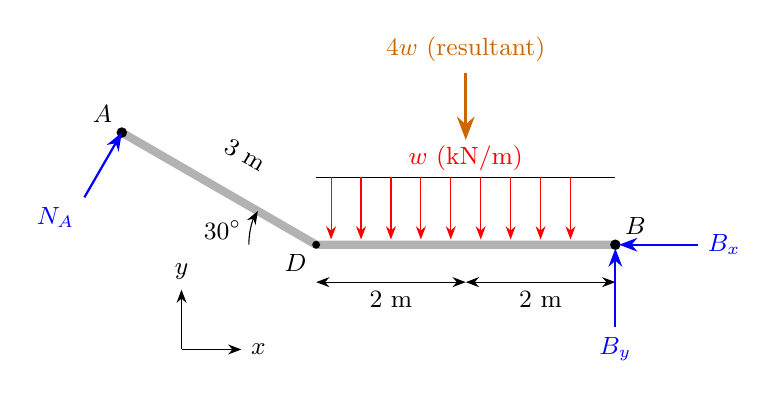
\begin{tikzpicture}[scale=0.95,>=Stealth,font=\small]
  \coordinate (A) at (-2.598,1.5);
  \coordinate (D) at (0,0);
  \coordinate (B) at (4,0);
  \draw[line width=3pt,gray!60] (A)--(D)--(B);
  \fill (A) circle(2pt) node[above left]{$A$};
  \fill (B) circle(2pt) node[above right]{$B$};
  \fill (D) circle(1.5pt) node[below left]{$D$};
  % distributed load
  \draw (0,0.9)--(4,0.9);
  \foreach \x in {0.2,0.6,...,3.8} \draw[->,red] (\x,0.9)--(\x,0.07);
  \node[red] at (2,1.15) {$w$ (kN/m)};
  \draw[->,very thick,orange!80!black] (2,2.3)--(2,1.4) node[pos=0,above]{$4w$ (resultant)};
  % reactions
  \draw[->,thick,blue] ($(A)+(-0.5,-0.866)$)--(A) node[pos=0,below left]{$N_A$};
  \draw[->,thick,blue] (4,-1.1)--(4,-0.05) node[pos=0,below]{$B_y$};
  \draw[->,thick,blue] (5.1,0)--(4.05,0) node[pos=0,right]{$B_x$};
  % dimensions
  \draw[<->] (0,-0.5)--(2,-0.5) node[midway,below]{2 m};
  \draw[<->] (2,-0.5)--(4,-0.5) node[midway,below]{2 m};
  \draw[->] (-0.9,0) arc (180:150:0.9); \node at (-1.25,0.2) {$30^\circ$};
  \node[rotate=-30] at (-0.95,1.2) {3 m};
  \draw[->] (-1.8,-1.4)--(-1.0,-1.4) node[right]{$x$};
  \draw[->] (-1.8,-1.4)--(-1.8,-0.6) node[above]{$y$};
\end{tikzpicture}
\end{center}

\textbf{Equations \& Solution:} The roller force $N_A$ is perpendicular to the incline. The distributed load becomes $4w$ at 2 m from $B$. The perpendicular distance from $B$ to the line of action of $N_A$ is $3 + 4\cos30^\circ = \SI{6.464}{m}$.
\begin{align*}
\sum M_B = 0:&\quad 4w(2) - N_A(6.464) = 0 \;\Rightarrow\; N_A = 1.238\,w\\
\sum F_x = 0:&\quad B_x = N_A\sin30^\circ = 0.619\,w\\
\sum F_y = 0:&\quad B_y = 4w - N_A\cos30^\circ = 2.928\,w\\
B &= \sqrt{B_x^2 + B_y^2} = 2.993\,w
\end{align*}
Roller: $1.238w \le 4 \Rightarrow w \le \SI{3.23}{kN/m}$. Pin: $2.993w \le 8 \Rightarrow w \le \SI{2.67}{kN/m}$. The pin governs.
\begin{finalanswer}
$w_{\max} = \SI{2.67}{kN/m}$ \quad (pin $B$ governs; roller carries $N_A = \SI{3.31}{kN} < \SI{4}{kN}$)
\end{finalanswer}

% =========================================================
% PROBLEM 3
% =========================================================
\probhead{3}{A 10 kg, 2 m uniform rod is pinned at $A$ and held by a horizontal spring ($k = \SI{60}{N/m}$, unstretched at $\theta = 0^\circ$) at $B$, with a \SI{50}{N.m} couple at $A$. Find the smallest $\theta$ for equilibrium.}

\begin{center}
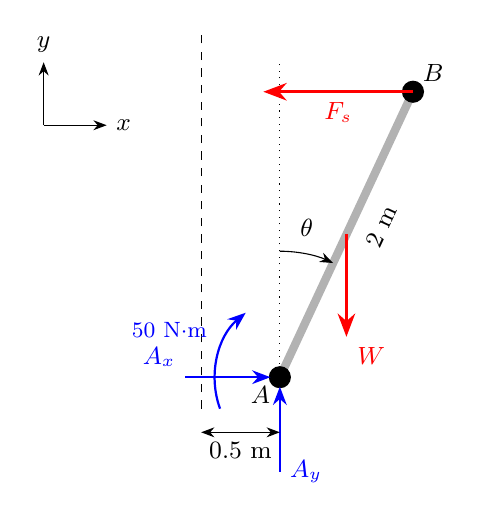
\begin{tikzpicture}[scale=2.0,>=Stealth,font=\small]
  \def\th{25}
  \pgfmathsetmacro{\bx}{2*sin(\th)}
  \pgfmathsetmacro{\by}{2*cos(\th)}
  \coordinate (A) at (0,0);
  \coordinate (B) at (\bx,\by);
  \draw[dashed] (-0.5,-0.2)--(-0.5,2.2);
  \draw[line width=3pt,gray!60] (A)--(B);
  \fill (A) circle(2pt) node[below left]{$A$};
  \fill (B) circle(2pt) node[above right]{$B$};
  \draw[dotted] (A)--(0,2.0);
  \draw[->] (0,0.8) arc (90:{90-\th}:0.8); \node at (0.17,0.95) {$\theta$};
  % spring force on rod, weight, reactions
  \draw[->,very thick,red] (B)--++(-0.95,0) node[pos=0.5,below]{$F_s$};
  \draw[->,very thick,red] ($(A)!0.5!(B)$)--++(0,-0.65) node[pos=1,below right]{$W$};
  \draw[->,thick,blue] (-0.6,0)--(-0.06,0) node[pos=0,above left]{$A_x$};
  \draw[->,thick,blue] (0,-0.6)--(0,-0.06) node[pos=0,right]{$A_y$};
  \draw[->,thick,blue] (-0.38,-0.2) arc (200:130:0.55);
  \node[blue,left] at (-0.4,0.3) {\footnotesize $50$ N$\cdot$m};
  % dims
  \draw[<->] (-0.5,-0.35)--(0,-0.35) node[midway,below]{0.5 m};
  \node[rotate=65] at (\bx/2+0.22,\by/2+0.05) {2 m};
  \draw[->] (-1.5,1.6)--(-1.1,1.6) node[right]{$x$};
  \draw[->] (-1.5,1.6)--(-1.5,2.0) node[above]{$y$};
\end{tikzpicture}
\end{center}

\textbf{Equations \& Solution:} Spring force (stretch is $2\sin\theta$) and weight:
\[ F_s = k(2\sin\theta) = 120\sin\theta\ \text{N}, \qquad W = (10)(9.81) = \SI{98.1}{N} \]
Moments about $A$ (spring force is ccw at height $2\cos\theta$; weight and couple are cw):
\begin{align*}
\sum M_A = 0:&\quad F_s(2\cos\theta) - W\sin\theta - 50 = 0\\
&\quad 120\sin2\theta - 98.1\sin\theta - 50 = 0
\end{align*}
Solved numerically, the roots are $24.6^\circ$ and $45.5^\circ$.
\begin{finalanswer}
$\theta_{\min} = 24.6^\circ$
\end{finalanswer}

% =========================================================
% PROBLEM 4
% =========================================================
\probhead{4}{Weightless bar, $d = \SI{1}{m}$, $\theta = 30^\circ$, resting on a smooth wall at its lower end and a smooth roller, with $P = \SI{600}{N}$ at the top. Find $N_w$, $N_r$, and $a$.}

\begin{center}
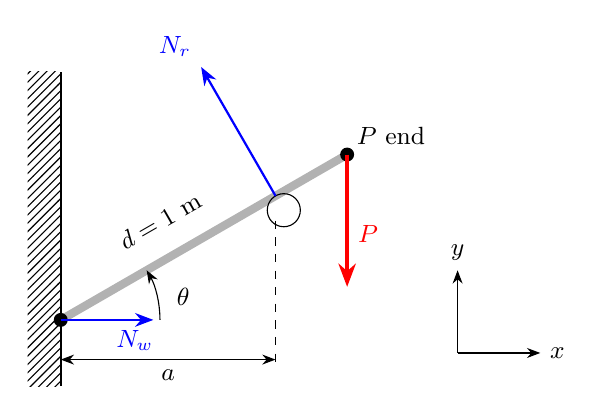
\begin{tikzpicture}[scale=4.2,>=Stealth,font=\small]
  \fill[pattern=north east lines] (-0.1,-0.2) rectangle (0,0.75);
  \draw[thick] (0,-0.2)--(0,0.75);
  \draw[line width=3pt,gray!60] (0,0)--(0.866,0.5);
  \fill (0,0) circle(0.6pt);
  \fill (0.866,0.5) circle(0.6pt) node[above right]{$P$ end};
  % roller at s = 0.75
  \draw (0.6495,0.375) ++(0.5*0.05,-0.866*0.05) circle(0.05);
  % forces
  \draw[->,very thick,red] (0.866,0.5)--++(0,-0.4) node[pos=0.6,right]{$P$};
  \draw[->,thick,blue] (0,0)--(0.28,0) node[pos=0.8,below]{$N_w$};
  \draw[->,thick,blue] (0.6495,0.375)--++(-0.5*0.45,0.866*0.45) node[above left]{$N_r$};
  % dims
  \draw[<->] (0,-0.12)--(0.6495,-0.12) node[midway,below]{$a$};
  \draw[dashed] (0.6495,0.3)--(0.6495,-0.15);
  \draw[->] (0.3,0) arc (0:30:0.3); \node at (0.37,0.07) {$\theta$};
  \node[rotate=30] at (0.3,0.3) {$d = 1$ m};
  \draw[->] (1.2,-0.1)--(1.45,-0.1) node[right]{$x$};
  \draw[->] (1.2,-0.1)--(1.2,0.15) node[above]{$y$};
\end{tikzpicture}
\end{center}

\textbf{Equations \& Solution:} $N_w$ is horizontal and $N_r$ is perpendicular to the bar. Let $s$ be the distance along the bar from the wall to the roller.
\begin{align*}
\sum F_y = 0:&\quad N_r\cos30^\circ = 600 \;\Rightarrow\; N_r = \SI{692.8}{N}\\
\sum F_x = 0:&\quad N_w = N_r\sin30^\circ = \SI{346.4}{N}\\
\sum M_{\text{wall}} = 0:&\quad N_r\,s - 600(1)\cos30^\circ = 0 \;\Rightarrow\; s = \SI{0.750}{m}\\
&\quad a = s\cos30^\circ = \SI{0.6495}{m}
\end{align*}
\begin{finalanswer}
$N_w = \SI{346}{N}$, \quad $N_r = \SI{693}{N}$, \quad $a = \SI{0.650}{m}$
\end{finalanswer}

% =========================================================
% PROBLEM 5
% =========================================================
\probhead{5}{Pipe assembly fixed at $A$ with 400 N (along $-x$), 500 N (along $+y$), and 600 N (down) applied as shown. Find the three force and three moment reactions at $A$.}

\begin{center}
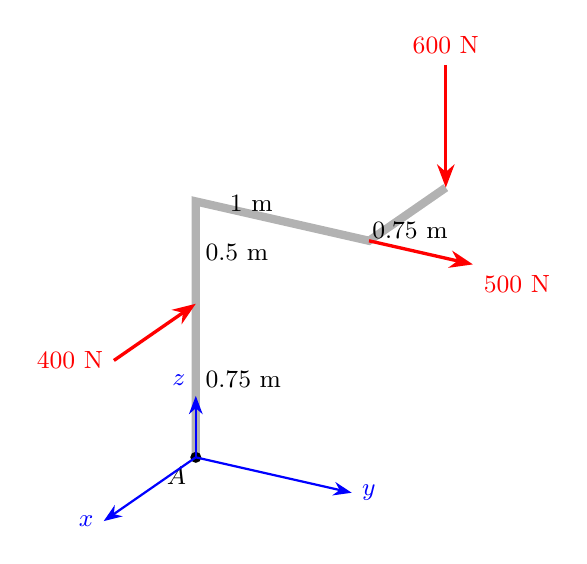
\begin{tikzpicture}[x={(-1.3cm,-0.9cm)},y={(2.2cm,-0.5cm)},z={(0cm,2.6cm)},>=Stealth,font=\small]
  % pipe
  \draw[line width=3pt,gray!60] (0,0,0)--(0,0,1.25)--(0,1,1.25)--(-0.75,1,1.25);
  \fill (0,0,0) circle(2pt);
  \node[below left] at (0,0,0) {$A$};
  % applied loads
  \draw[->,very thick,red] (0.8,0,0.75)--(0,0,0.75) node[pos=0,left]{400 N};
  \draw[->,very thick,red] (0,1,1.25)--(0,1.6,1.25) node[below right]{500 N};
  \draw[->,very thick,red] (-0.75,1,1.85)--(-0.75,1,1.25) node[pos=0,above]{600 N};
  % reactions / axes at A
  \draw[->,thick,blue] (0,0,0)--(0.9,0,0) node[left]{$x$};
  \draw[->,thick,blue] (0,0,0)--(0,0.9,0) node[right]{$y$};
  \draw[->,thick,blue] (0,0,0)--(0,0,0.3) node[above left]{$z$};
  % dimensions
  \node[right] at (0,0,0.38) {0.75 m};
  \node[right] at (0,0,1.0) {0.5 m};
  \node[above left] at (0,0.5,1.25) {1 m};
  \node[below] at (-0.4,1,1.25) {0.75 m};
\end{tikzpicture}
\end{center}

\textbf{Equations \& Solution:} Positions from $A$ (m) and applied forces (N):
\begin{align*}
\mathbf{r}_1 &= \langle 0,0,0.75\rangle, & \mathbf{F}_1 &= \langle -400,0,0\rangle\\
\mathbf{r}_2 &= \langle 0,1,1.25\rangle, & \mathbf{F}_2 &= \langle 0,500,0\rangle\\
\mathbf{r}_3 &= \langle -0.75,1,1.25\rangle, & \mathbf{F}_3 &= \langle 0,0,-600\rangle
\end{align*}
Forces: $\mathbf{A} = -\sum\mathbf{F} = \langle 400, -500, 600\rangle$ N.

Moments: $\mathbf{M}_A = -\sum \mathbf{r}\times\mathbf{F}$, with
\[ \mathbf{r}_1\times\mathbf{F}_1 = \langle 0,-300,0\rangle,\quad \mathbf{r}_2\times\mathbf{F}_2 = \langle -625,0,0\rangle,\quad \mathbf{r}_3\times\mathbf{F}_3 = \langle -600,-450,0\rangle\ \text{N.m} \]
so $\mathbf{M}_A = \langle 1225, 750, 0\rangle$ N.m.
\begin{finalanswer}
$A_x = \SI{400}{N}$, \; $A_y = \SI{-500}{N}$, \; $A_z = \SI{600}{N}$\\
$M_x = \SI{1.23}{kN.m}$, \; $M_y = \SI{750}{N.m}$, \; $M_z = 0$
\end{finalanswer}

% =========================================================
% PROBLEM 6
% =========================================================
\probhead{6}{A 2400 kg uniform slab hangs from three vertical cables at $A$, $B$, $C$ with an additional 15 kN load on it. Find $T_A$, $T_B$, $T_C$.}
 
\begin{center}
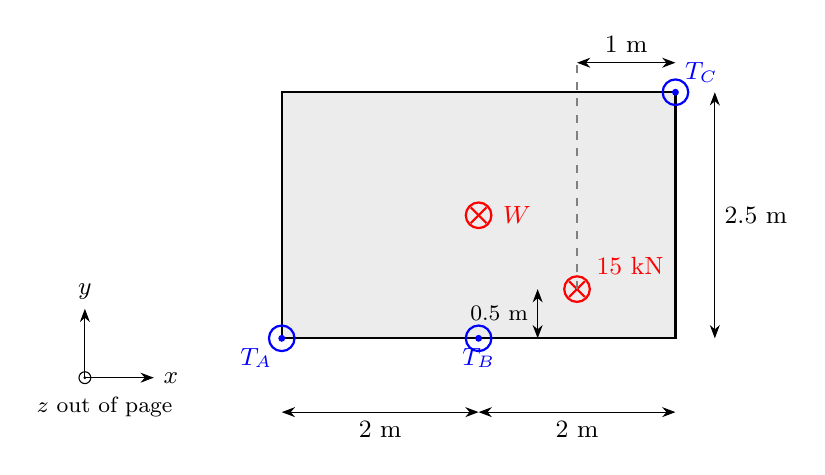
\begin{tikzpicture}[scale=1.25,>=Stealth,font=\small]
  % plan view: x to the right, y up, z out of page (right-handed); origin at A
  \draw[thick,fill=gray!15] (0,0) rectangle (4,2.5);
  \foreach \p/\n/\a in {(0,0)/A/below left, (2,0)/B/below, (4,2.5)/C/above right}{
     \draw[blue,thick] \p circle(0.13); \fill[blue] \p circle(0.035);
     \node[blue,\a] at \p {$T_\n$};
  }
  % 15 kN load (into page) at (x,y) = (3,0.5)
  \draw[red,thick] (3,0.5) circle(0.13); \draw[red,thick] (2.92,0.42)--(3.08,0.58); \draw[red,thick] (2.92,0.58)--(3.08,0.42);
  \node[red,above right] at (3.1,0.55) {15 kN};
  % weight at centroid (2,1.25)
  \draw[red,thick] (2,1.25) circle(0.13); \draw[red,thick] (1.92,1.17)--(2.08,1.33); \draw[red,thick] (1.92,1.33)--(2.08,1.17);
  \node[red,right] at (2.15,1.25) {$W$};
  % axes (origin at A, drawn offset)
  \draw[->] (-2.0,-0.4)--(-1.3,-0.4) node[right]{$x$};
  \draw[->] (-2.0,-0.4)--(-2.0,0.3) node[above]{$y$};
  \draw (-2.0,-0.4) circle(0.06); \fill (-2.0,-0.4) circle(0.015);
  \node[font=\footnotesize,below] at (-1.8,-0.5) {$z$ out of page};
  % dims
  \draw[<->] (0,-0.75)--(2,-0.75) node[midway,below]{2 m};
  \draw[<->] (2,-0.75)--(4,-0.75) node[midway,below]{2 m};
  \draw[<->] (4.4,0)--(4.4,2.5) node[midway,right]{2.5 m};
  \draw[<->] (3,2.8)--(4,2.8) node[midway,above]{1 m};
  \draw[dashed,gray] (3,0.5)--(3,2.8);
  \draw[<->] (2.6,0)--(2.6,0.5) node[midway,left,font=\footnotesize]{0.5 m};
\end{tikzpicture}
\end{center}
 
\textbf{Equations \& Solution:} Dimensions read from the figure: slab $4\times2.5$ m with origin at $A$. $A(0,0)$, $B(2,0)$, $C(4,2.5)$, 15 kN load at $(3,0.5)$, centroid at $(2,1.25)$ m. $W = (2400)(9.81) = \SI{23.54}{kN}$.
\begin{align*}
\sum F_z = 0:&\quad T_A + T_B + T_C = 23.54 + 15 = 38.54\\
\sum M_x = 0:&\quad 2.5\,T_C = 23.54(1.25) + 15(0.5) \;\Rightarrow\; T_C = \SI{14.77}{kN}\\
\sum M_y = 0:&\quad 2T_B + 4T_C = 23.54(2) + 15(3) \;\Rightarrow\; T_B = \SI{16.50}{kN}
\end{align*}
Then $T_A = 38.54 - 16.50 - 14.77 = \SI{7.27}{kN}$.
\begin{finalanswer}
$T_A = \SI{7.27}{kN}$, \quad $T_B = \SI{16.5}{kN}$, \quad $T_C = \SI{14.8}{kN}$
\end{finalanswer}

\end{document}